\section{ХОД РАБОТЫ}

\subsection{Формулировка задачи}

Требуется вывести на экран монитора графики поверхностей и линии равных
уровней плотностей вероятности приведенных выше двухмерных распределений
(при $ k = 2 $ ) и исследовать их зависимость от параметров распределений.

Для нормального распределения в одно графическое окно вывести эллипс
рассеяния и две функции регрессии. Исследовать зависимость формы и
площади эллипса рассеяния от коэффициента корреляции при заданных дисперсиях
компонент случайного вектора. Исследовать взаимное расположение
функций регрессии и осей эллипса рассеяния (совпадают ли функции регрессии
с осями эллипса?).

\subsection{Теоретические сведения}

Приведём формулы, которые будут использованы для построения графиков.

Плотность вероятности \textit{произведения одномерных гамма-распределений}:
\begin{equation}
    \begin{aligned}
      f_{\overline{\xi}}(\overline{x}) =
      \left\{
        \begin{aligned}
          &\prod_{i=1}^m \dfrac{1}{\Gamma(a_i)b_i^{a_i}} x_i^{a_i-1} e^{-\dfrac{x_i}{b_i}}, \hspace{3mm} &x_i > 0, b_i > 0, a_i > 0, \\
          &0, \hspace{11.5mm} &x \le a.
        \end{aligned}
      \right.
    \end{aligned}
  \end{equation}

Плотность вероятности \textit{двухмерного нормального распределения}:
\begin{equation}
    \begin{aligned}
      f_{\overline{\xi}}(x_1, x_2) =
      \left\{
        \begin{aligned}
          \dfrac{1}{2 \pi \sigma_1 \sigma_2 \sqrt{1-r_{1,2}^2}} \hspace{1mm} exp \Big(-\dfrac{1}{2}\phi(x_1, x_2) \Big).
        \end{aligned}
      \right.
    \end{aligned}
  \end{equation}

\newpage
\subsection{Многомерное нормальное распределение}

Графики поверхностей двухмерного нормального распределения представлены
на рисунках~\ref{pic:normal_mesh_start}~-~\ref{pic:normal_mesh_end}.

\begin{figure}[h]
  \begin{minipage}[h]{0.49\linewidth}
    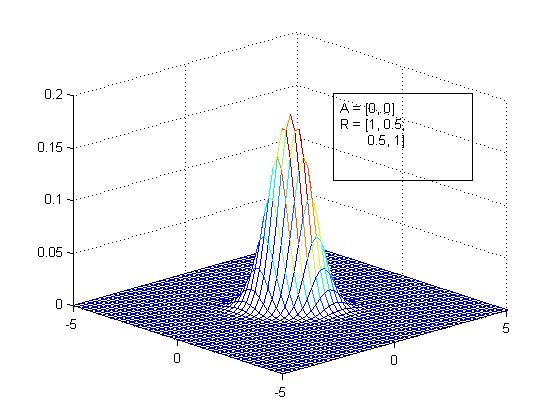
\includegraphics[width=1\linewidth]{../pic/new/normal_mesh_1}
    \caption{График поверхностей двухмерного нормального распределения при}
    \label{pic:normal_mesh_start}
  \end{minipage}
  \hfill
  \begin{minipage}[h]{0.49\linewidth}
    \vspace{4mm}
    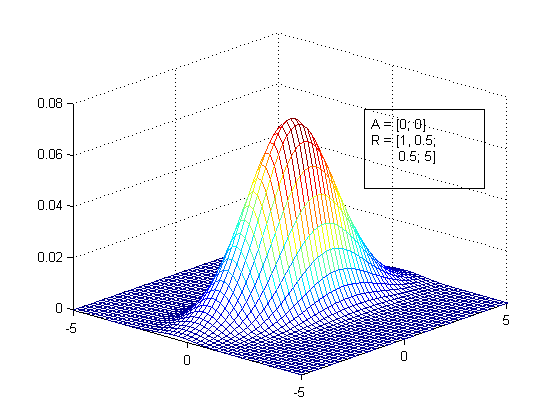
\includegraphics[width=1\linewidth]{../pic/new/normal_mesh_2}
    \caption{График поверхностей двухмерного нормального распределения при}
  \end{minipage}
\end{figure}

\begin{figure}[h]
  \begin{minipage}[h]{0.49\linewidth}
    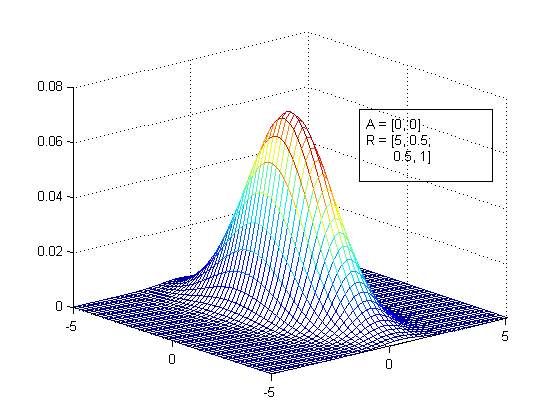
\includegraphics[width=1\linewidth]{../pic/new/normal_mesh_3}
    \caption{График поверхностей двухмерного нормального распределения при}
  \end{minipage}
  \hfill
  \begin{minipage}[h]{0.49\linewidth}
    \vspace{4mm}
    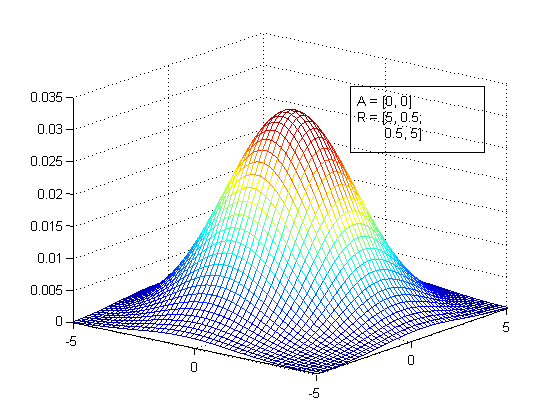
\includegraphics[width=1\linewidth]{../pic/new/normal_mesh_4}
    \caption{График поверхностей двухмерного нормального распределения при}
    \label{pic:normal_mesh_end}
  \end{minipage}
\end{figure}

\newpage

Графики линий равных уровней плотности вероятности нормального распределения при различных
параметрах приведены на рисунках~\ref{pic:normal_contour_start}~-~\ref{pic:normal_contour_end}.

\begin{figure}[h]
  \begin{minipage}[h]{0.49\linewidth}
    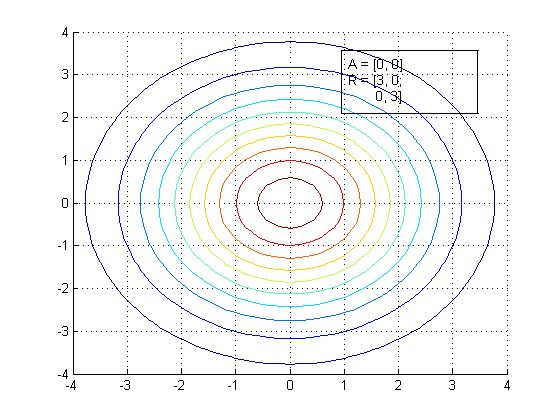
\includegraphics[width=1\linewidth]{../pic/new/normal_contour_1}
    \caption{Графики линий равных уровней плотности вероятности нормального распределения при }
    \label{pic:normal_contour_start}
  \end{minipage}
  \hfill
  \begin{minipage}[h]{0.49\linewidth}
    \vspace{4mm}
    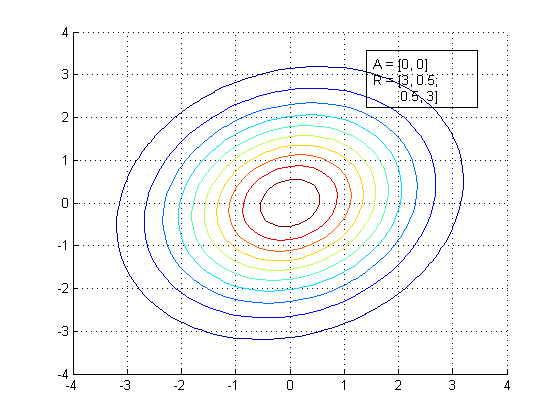
\includegraphics[width=1\linewidth]{../pic/new/normal_contour_2}
    \caption{Графики линий равных уровней плотности вероятности нормального распределения при }
  \end{minipage}
\end{figure}

\begin{figure}[h]
  \centering
  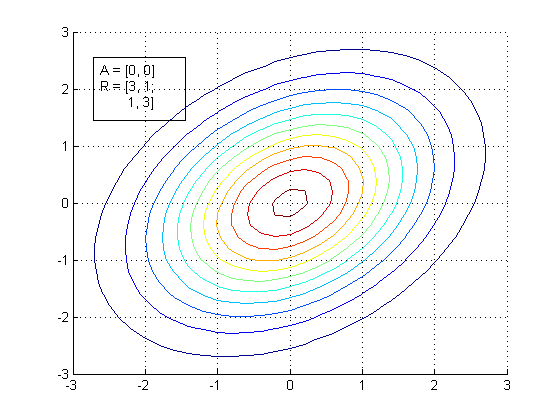
\includegraphics[width=0.58\linewidth]{../pic/new/normal_contour_3}
  \caption{Графики линий равных уровней плотности вероятности нормального распределения при }
  \label{pic:normal_contour_end}
\end{figure}

\newpage

\subsection{Произведение одномерных гамма-распределений}

Графики поверхностей произведения одномерных гамма-распределений продемонстрированы
на рисунках~\ref{pic:gamma_mesh_start}~-~\ref{pic:gamma_mesh_end}.

\begin{figure}[h]
  \begin{minipage}[h]{0.49\linewidth}
    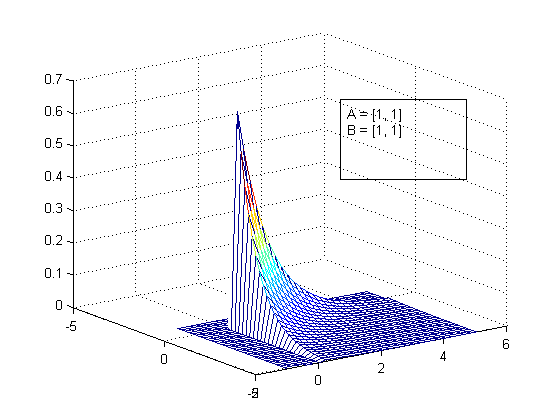
\includegraphics[width=1\linewidth]{../pic/new/gamma_mesh_1}
    \caption{График поверхности произведения одномерных гамма-распределений при }\label{pic:gamma_mesh_start}
  \end{minipage}
  \hfill
  \begin{minipage}[h]{0.49\linewidth}
    \vspace{4mm}
    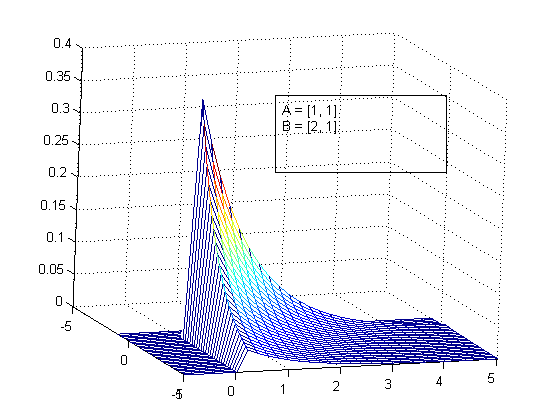
\includegraphics[width=1\linewidth]{../pic/new/gamma_mesh_2}
    \caption{График поверхности произведения одномерных гамма-распределений при }
  \end{minipage}
\end{figure}

\begin{figure}[h]
  \begin{minipage}[h]{0.49\linewidth}
    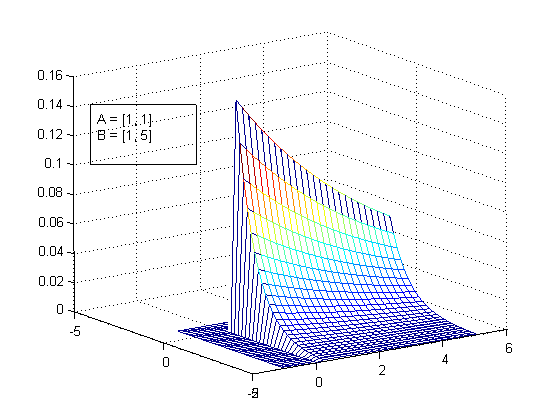
\includegraphics[width=1\linewidth]{../pic/new/gamma_mesh_3}
    \caption{График поверхности произведения одномерных гамма-распределений при}
  \end{minipage}
  \hfill
  \begin{minipage}[h]{0.49\linewidth}
    \vspace{4mm}
    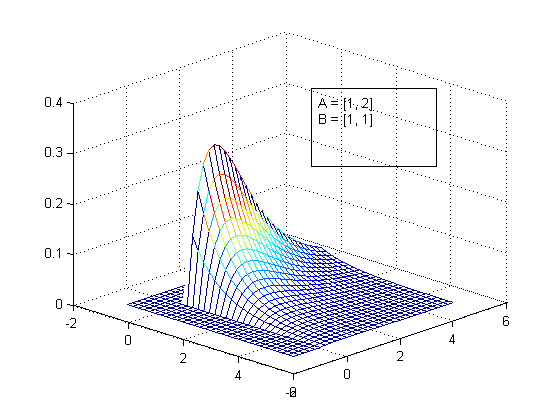
\includegraphics[width=1\linewidth]{../pic/new/gamma_mesh_4}
    \caption{График поверхности произведения одномерных гамма-распределений при}
  \end{minipage}
\end{figure}

\newpage

\begin{figure}[h]
  \begin{minipage}[h]{0.49\linewidth}
    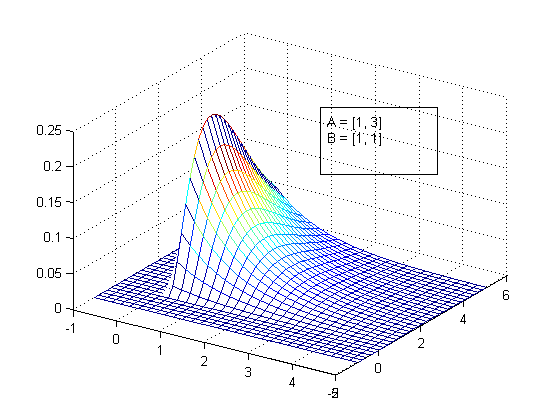
\includegraphics[width=1\linewidth]{../pic/new/gamma_mesh_5}
    \caption{График поверхности произведения одномерных гамма-распределений при }
  \end{minipage}
  \hfill
  \begin{minipage}[h]{0.49\linewidth}
    \vspace{4mm}
    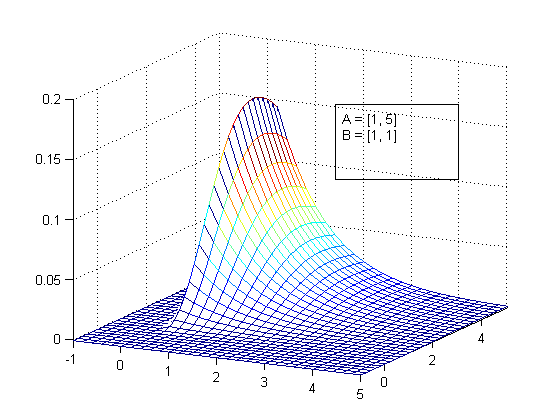
\includegraphics[width=1\linewidth]{../pic/new/gamma_mesh_6}
    \caption{График поверхности произведения одномерных гамма-распределений при}
  \end{minipage}
\end{figure}

\begin{figure}[h]
  \centering
  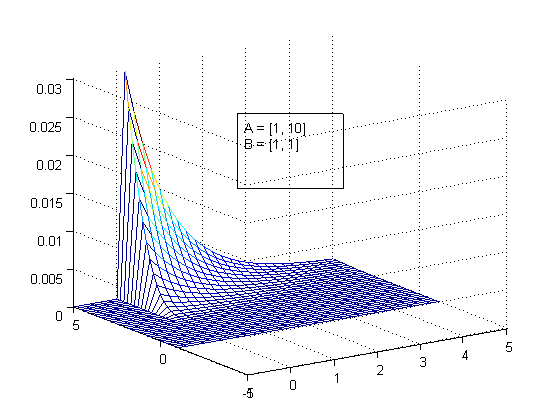
\includegraphics[width=0.58\linewidth]{../pic/new/gamma_mesh_7}
  \caption{График поверхности произведения одномерных гамма-распределений при}\label{pic:gamma_mesh_end}
\end{figure}

\newpage

Графики линий равных уровней плотности вероятности гамма-распределений при различных
параметрах приведены на рисунках~\ref{pic:gamma_contour_start}~-~\ref{pic:gamma_contour_end}.

\begin{figure}[h]
  \begin{minipage}[h]{0.49\linewidth}
    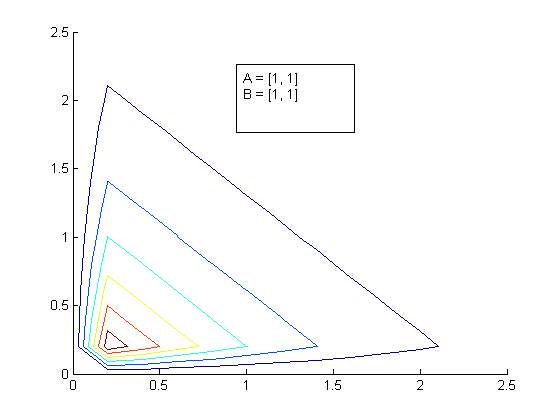
\includegraphics[width=1\linewidth]{../pic/gamma_contour_1}
    \caption{График линий уровней плотности вероятности гамма-распределений при}
    \label{pic:gamma_contour_start}
  \end{minipage}
  \hfill
  \begin{minipage}[h]{0.49\linewidth}
    \vspace{4mm}
    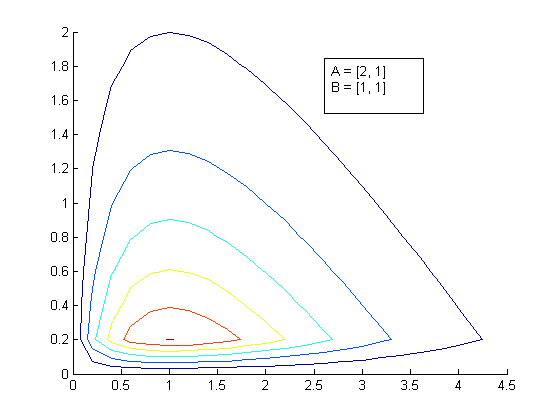
\includegraphics[width=1\linewidth]{../pic/gamma_contour_2}
    \caption{График линий уровней плотности вероятности гамма-распределений при}
  \end{minipage}
\end{figure}

\begin{figure}[h]
  \centering
  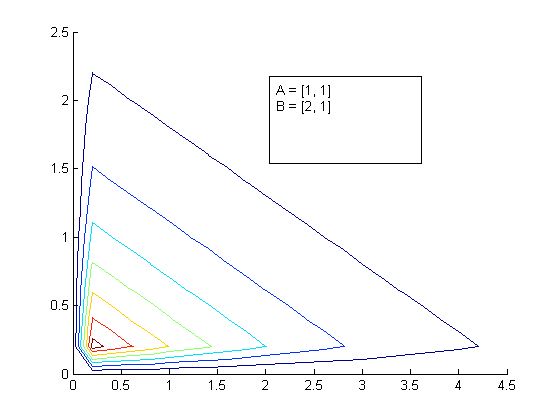
\includegraphics[width=0.58\linewidth]{../pic/gamma_contour_3}
  \caption{График линий уровней плотности вероятности гамма-распределений при}
  \label{pic:gamma_contour_end}
\end{figure}

\newpage

\subsection{Эллипс рассеяния и две функции регрессии}

Графики эллипса рассеяния и две функции регрессии при различных параметрах
представлены на рисунках~\ref{pic:normal_regr_start}~-~\ref{pic:normal_regr_end}.

\begin{figure}[h]
  \begin{minipage}[h]{0.49\linewidth}
    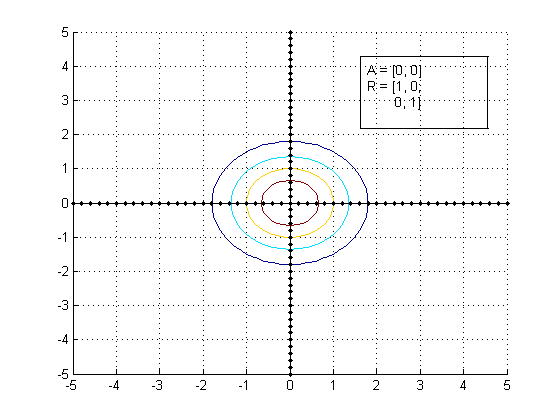
\includegraphics[width=1\linewidth]{../pic/new/normal_regr_1}
    \caption{График эллипса рассеяния и двух функций регрессии при}\label{pic:normal_regr_start}
  \end{minipage}
  \hfill
  \begin{minipage}[h]{0.49\linewidth}
    \vspace{4mm}
    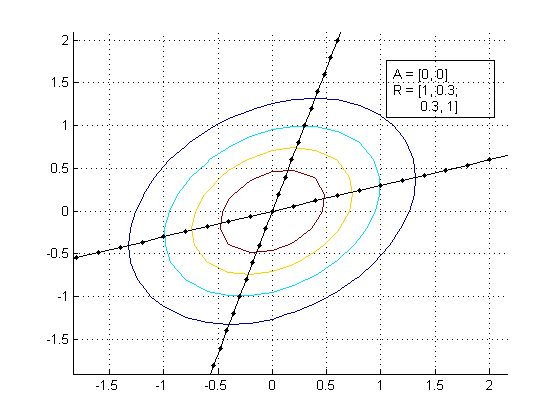
\includegraphics[width=1\linewidth]{../pic/new/normal_regr_2}
    \caption{График эллипса рассеяния и двух функций регрессии при}
  \end{minipage}
\end{figure}

\begin{figure}[h]
  \begin{minipage}[h]{0.49\linewidth}
    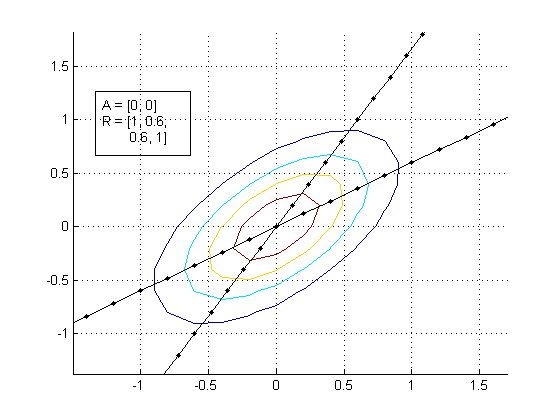
\includegraphics[width=1\linewidth]{../pic/new/normal_regr_3}
    \caption{График эллипса рассеяния и двух функций регрессии при}
  \end{minipage}
  \hfill
  \begin{minipage}[h]{0.49\linewidth}
    \vspace{4mm}
    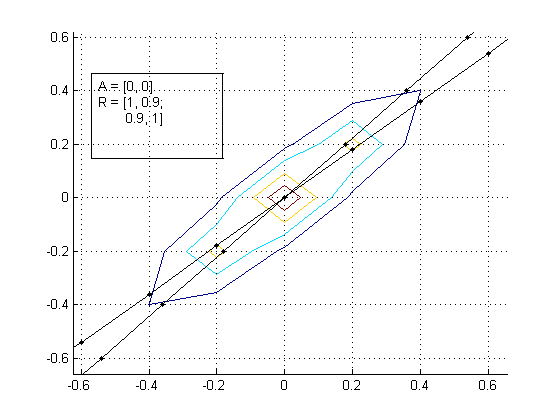
\includegraphics[width=1\linewidth]{../pic/new/normal_regr_4}
    \caption{График эллипса рассеяния и двух функций регрессии при}
  \end{minipage}
\end{figure}

\begin{figure}[h]
  \centering
  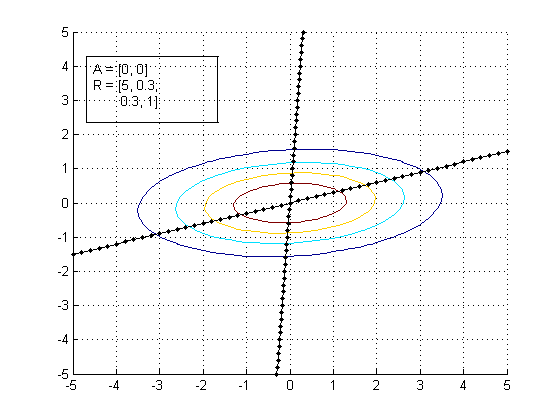
\includegraphics[width=0.6\linewidth]{../pic/new/normal_regr_5}
  \caption{График эллипса рассеяния и двух функций регрессии при}\label{pic:normal_regr_end}
\end{figure}

\newpage
